\documentclass[12pt]{article}

\usepackage{amsmath,amssymb,amsthm}
\usepackage[T1]{fontenc}
\usepackage{graphics}
\usepackage{qtree}
\usepackage{tikz}
\usepackage[utf8]{inputenc} % æøå
\usepackage[T1]{fontenc} % mere æøå
\usepackage[danish]{babel} % orddeling
\usepackage{verbatim} % så man kan skrive ren tekst
\usepackage[all]{xy} % den sidste (avancerede) formel i dokumentet
\usepackage{fullpage} % mindre margin

\title{ProjDat 2014\\Props 2.0}
\author{Louise Knudsen (140791 - zsh845)\\
Helena Bach (180492 - wzg314)\\
David Pedersen (060890 - tlb209)\\\\
Instructor: Simon Shine }
\date{\today}

\newcommand{\R}{\mathbb{R}}
\newcommand{\C}{\mathbb{C}}
\newcommand{\N}{\mathbb{N}}
\newcommand{\Z}{\mathbb{Z}}
\newcommand{\Q}{\mathbb{Q}}

\newcommand{\og}{\wedge}

\begin{document}
\maketitle
\newpage
\section{Abstract}
\textit{The Royal Danish Theatre's props department uses a locally installed database-system to search through all of the props and productions and their corresponding set-up- and run-lists. The system was developed more than 20 years ago by their own Claus Nepper Fakkenberg. Claus alone holds the responsibility for maintaining the system, as he is the only one who understands the source-code, which will soon be a problem as he is now retiring. \\
Due to the age of the system, some functionalities are no longer needed, and there are new requirements that are not implemented, most importantly a need to use the system outside of the office. Our project will therefore be to develop a web-based database-system for the props department, to replace the current system.}
\section{Project purpose and scope}
A web-based database-system of The Royal Danish Theatre props department. The system should primarily be a searching tool used to prepare and run performances and search for props in current and previous productions by the assistant stage managers, and secondly be used for budget monitoring, search for supplier information as well as keeping track of all performance information, by the chairman of the props department. The system should be usable for people with greatly variable computer experience.
\subsection{The FACTOR Criterion}
\begin{description}
  \item[Functionality:] Keeping track of the props and performances, and help in running these. As well as support the administration.
  \item[Application domain:] The Royal Danish Theatre.
  \item[Conditions:] The system should be usable by multiple user at a time, wherever there are access to the internet.
  \item[Technology:] The system will be developed on standard laptops, and should be usable on standard PC's and tablets and supported by every OS.
  \item[Object:] Props, pictures and employees in the props department.
  \item[Responsibility:] Searching and administrative tool.
\end{description}
\section{Requirement Elicitation}
\subsection{a)}
\subsubsection{Nonfunctional Requirements}
\begin{itemize}
  \item The system should be web-based and usable on standard PC's and tablets, and supported by every OS.
  \item The webapplication should be user friendly and easy to navigate. The most commonly used functionalities, namely the run- and set-up-lists should be preferable be found on the frontpage.
  \item It should be possible for Martin (head of the IT-department) to maintain and support, and possibly expand the system after product-delivery. Therefore the system will be developed using MySQL and PHP, which is familiar to Martin.
  \item The system should be able to communicate with the existing media-database Cumulus.
  \item The system should be secure in a way that prevents people from the outside to corrupt the data.
  \item The interface should be in Danish.
  \item It should be made in such a way that makes it easy to extend with additonal functionality.
\end{itemize}
\subsubsection{Functional Requirements}
\begin{itemize}
  \item It should be possible to do cross search for props, productions, and suppliers.
  \item It should be possible to add, edit and delete props, productions, and suppliers.
  \item It should be possible to print run- and set-up-lists.
\end{itemize}
\subsection{b) UML use case diagram}
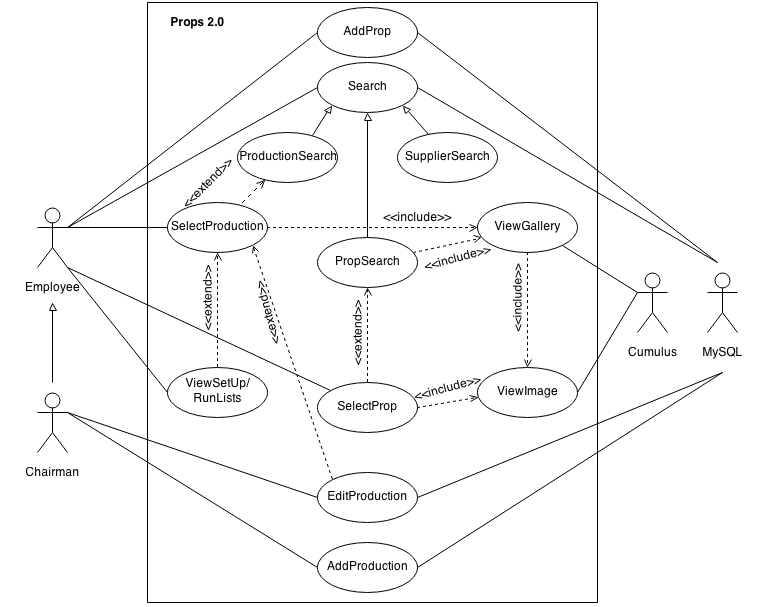
\includegraphics[scale=0.6]{use.png}
\subsection{c) Use cases}
The following three use cases are the ones of most importance:
%1. Tilføj Rek
\[
\begin{array}{ll}
\hline
\textit{Use case name} & \texttt{AddProp} \\
\hline
\textit{Participating actors} & \text{Initiated by \texttt{Employee}} \\
& \text{Communicates with \texttt{MySQL}} \\
\hline
\textit{Flow of events} & 
\begin{array}{l}
\text{1. The \texttt{Employee} activates the "Add prop"  function.}\\
\quad \quad \quad \text{2. \texttt{Props 2.0} responds by presenting a form to the \texttt{Employee}.} \\
\text{3. The \texttt{Employee} fills out the form with the relevant prop-info,} \\ \quad \text{and submits it.} \\
\quad \quad \quad \text{4. \texttt{Props 2.0} receives the form, and the MySQL database} \\ \quad \quad \quad \quad \text{gets updated. \texttt{Props 2.0} displays a confirmation of the}\\ \quad \quad \quad \quad \text{update.}
\end{array} \\
\hline
\textit{Entry condition} & \text{The \texttt{Employee} must be logged into the Theatre's Wi-Fi} \\
\hline
\textit{Exit condition} & \text{The \texttt{Employee} has received a confirmation OR} \\ & \text{An explanation indicating why the transaction could not be processed.} \\
\hline
\textit{Quality requirements} & \text{Not yet defined} \\
\hline
\end{array}
\]
%2. Tilføj forestilling
\\\\
\[
\begin{array}{ll}
\hline
\textit{Use case name} & \texttt{AddProduction} \\
\hline
\textit{Participating actors} & \text{Initiated by \texttt{Chairman}} \\
& \text{Communicates with \texttt{MySQL}} \\
\hline
\textit{Flow of events} & 
\begin{array}{l}
\text{1. The \texttt{Chairman} activates the "Add production" function.}\\
\quad \quad \quad \text{2. \texttt{Props 2.0} responds by presenting a form to the \texttt{Chairman}.} \\
\text{3. The \texttt{Chairman} fills out the form with the relevant production-info,} \\ \quad \text{and submits it.} \\
\quad \quad \quad \text{4. \texttt{Props 2.0} receives the form, and the MySQL database} \\ \quad \quad \quad \quad \text{gets updated. \texttt{Props 2.0} displays a confirmation of the}\\ \quad \quad \quad \quad \text{update.}
\end{array} \\
\hline
\textit{Entry condition} & \text{The \texttt{Chairman} must be logged into the Theatre's Wi-Fi} \\
\hline
\textit{Exit condition} & \text{The \texttt{Chairman} has received a confirmation OR} \\ & \text{An explanation indicating why the transaction could not be processed.} \\
\hline
\textit{Quality requirements} & \text{Not yet defined}\\
\hline
\end{array}
\]
%3. Søg
\\\\
\[
\begin{array}{ll}
\hline
\textit{Use case name} & \texttt{Search} \\
\hline
\textit{Participating actors} & \text{Initiated by \texttt{Employee}} \\
& \text{Communicates with \texttt{MySQL}} \\
\hline
\textit{Flow of events} & 
\begin{array}{l}
\text{1. The \texttt{Employee} activates the "Search" function.}\\
\quad \quad \quad \text{2. \texttt{Props 2.0} responds by presenting a form to the \texttt{Employee}.} \\
\text{3. The \texttt{Employee} fills out the form with the search criteria,} \\ \quad \text{and submits it.} \\
\quad \quad \quad \text{4. \texttt{Props 2.0} receives the form, the MySQL database} \\ \quad \quad \quad \quad \text{returns the matching data and \texttt{Props 2.0} displays it}
\end{array} \\
\hline
\textit{Entry condition} & \text{The \texttt{Employee} must be logged into the Theatre's Wi-Fi} \\
\hline
\textit{Exit condition} & \text{The \texttt{Employee} has received a list of matching data OR} \\ & \text{A "No match"  message} \\
\hline
\textit{Quality requirements} & \text{Not yet defined} \\
\hline
\end{array}
\]
%4. Vælg rek
\\
We have in addition made use cases, explaining the rest of the actions in the UML use case diagram: \\
\[
\begin{array}{ll}
\hline
\textit{Use case name} & \texttt{SelectProp} \\
\hline
\textit{Participating actors} & \text{Initiated by \texttt{Employee}} \\
\hline
\textit{Flow of events} & 
\begin{array}{l}
\text{1. The \texttt{Employee} selects a prop from the results of a premade search} \\
\quad \quad \quad \text{2. \texttt{Props 2.0} responds by presenting a more detailed}\\ \quad \quad \quad \quad \text{description of the prop to the \texttt{Employee}.}
\end{array} \\
\hline
\textit{Entry condition} & \text{This use case extends the  \texttt{PropSearch} use case} \\
\hline
\textit{Exit condition} & \text{The \texttt{Employee} is looking at the prop description} \\
\hline
\textit{Quality requirements} & \text{This use case includes the \texttt{ViewImage} use case} \\
\hline
\end{array}
\]
%5. Vælg forestilling:\\
\\\\
\[
\begin{array}{ll}
\hline
\textit{Use case name} & \texttt{SelectProduction} \\
\hline
\textit{Participating actors} & \text{Initiated by \texttt{Employee}} \\
\hline
\textit{Flow of events} & 
\begin{array}{l}
\text{1. The \texttt{Employee} selects a production from the results of a premade}\\ \quad \text{search}\\
\quad \quad \quad \text{2. \texttt{Props 2.0} responds by presenting a more detailed}\\
\quad \quad \quad \quad \text{description of the production to the \texttt{Employee}.}
\end{array} \\
\hline
\textit{Entry condition} &
\text{This use case extends the \texttt{ProductionSearch} use case.}\\
\hline
\textit{Exit condition} & \text{The \texttt{Employee} is looking at the production information.} \\
\hline
\textit{Quality requirements} & \text{This use case includes the \texttt{ViewGallery} use case.} \\
\hline
\end{array}
\]
%6. Køre/opstil
\\\\
\[
\begin{array}{ll}
\hline
\textit{Use case name} & \texttt{ViewSetUp/RunLists} \\
\hline
\textit{Participating actors} & \text{Initiated by \texttt{Employee}} \\
\hline
\textit{Flow of events} & 
\begin{array}{l}
\text{1. The \texttt{Employee} selects the list from the results of a production} \\ \quad \text{search} \\
\quad \quad \quad \text{2. \texttt{Props 2.0} responds by presenting the list to the}\\ \quad \quad \quad \quad \texttt{Employee.}
\end{array} \\
\hline
\textit{Entry condition} & \text{This use case extends the  \texttt{SelectProduction} use case} \\
\hline
\textit{Exit condition} & \text{The \texttt{Employee} is looking at the list} \\
\hline
\textit{Quality requirements} & \text{Not yet defined} \\
\hline
\end{array}
\]
%7. Redigér/slet
\\\\
\[
\begin{array}{ll}
\hline
\textit{Use case name} & \texttt{EditProduction} \\
\hline
\textit{Participating actors} & \text{Initiated by \texttt{Chairman}} \\
& \text{Communitates with \texttt{MySQL}} \\
\hline
\textit{Flow of events} & 
\begin{array}{l}
\text{1. The \texttt{Chairman} activates the "Edit production" function} \\
\quad \quad \quad \text{2. \texttt{Props 2.0} responds by presenting a form to the \texttt{Chairman}}\\
\text{3. The \texttt{Chairman} fills out the form and submit the changes OR} \\ \quad \text{The \texttt{Chairman} selects the "Delete" option} \\
\quad \quad \quad \text{4. \texttt{Props 2.0} receives the form, and the MySQL database} \\ \quad \quad \quad \quad \text{gets updated. \texttt{Props 2.0} displays a update- OR}\\\quad \quad \quad \quad \text{delete-comfirmation} 
\end{array} \\
\hline
\textit{Entry condition} & \text{This use case extends the  \texttt{SelectProduction} use case} \\
\hline
\textit{Exit condition} & \text{The \texttt{Chairman} has received a confirmation OR} \\ & \text{An explanation indicating why the transaction could not be processed.} \\
\hline
\textit{Quality requirements} & \text{Not yet defined} \\
\hline
\end{array}
\]
%8. Se Galleri:
\\\\
\[
\begin{array}{ll}
\hline
\textit{Use case name} & \texttt{ViewGallery} \\
\hline
\textit{Participating actors} & \text{Initiated by \texttt{Employee}}\\ &
\text{Communicates with \texttt{Cumulus}}\\
\hline
\textit{Flow of events} & 
\begin{array}{l}
\text{1. The \texttt{SelectProduction} or \texttt{PropSearch} use case gets evoked}\\
\quad \quad \quad \text{2. \texttt{Props 2.0} requests \texttt{Cumulus} for the image data}\\
3.\text{\texttt{Cumulus} returns the matching images}\\
\quad \quad \quad \text{4. \texttt{Props 2.0} responds by presenting the images as a gallery}
\end{array} \\
\hline
\textit{Entry condition} &
\text{The \texttt{Employee} must initiate the \texttt{SelectProduction} or \texttt{PropSearch}}\\ &
\text{use case to initiate this use case}\\
\hline
\textit{Exit condition} & \text{The \texttt{Employee} is looking at the gallery.} \\
\hline
\textit{Quality requirements} & \text{This use case includes the \texttt{ViewImage} use case.} \\
\hline
\end{array}
\]
%9. Se billede:
\\\\
\[
\begin{array}{ll}
\hline
\textit{Use case name} & \texttt{ViewImage} \\
\hline
\textit{Participating actors} & \text{Initiated by \texttt{Employee}}\\ &
\text{Communicates with \texttt{Cumulus}}\\
\hline
\textit{Flow of events} & 
\begin{array}{l}
\text{1. The \texttt{ViewGallery} or \texttt{SelectProp} use case gets evoked}\\
\quad \quad \quad \text{2. \texttt{Props 2.0} requests \texttt{Cumulus} for the image}\\
\text{3. \texttt{Cumulus} returns the matching image}\\
\quad \quad \quad \text{4. \texttt{Props 2.0} responds by presenting the image to the}\\ \quad \quad \quad \quad\texttt{Employee}
\end{array} \\
\hline
\textit{Entry condition} &
\text{The \texttt{Employee} must initiate the \texttt{ViewGallery} or \texttt{SelectProp} use}\\ &
\text{case to initiate this use case}\\
\hline
\textit{Exit condition} & \text{The \texttt{Employee} is looking at the image.} \\
\hline
\textit{Quality requirements} & \text{Not yet defined} \\
\hline
\end{array}
\]
\subsection{d) Class diagram}
Here is a class diagram of the model layer as we imagine it might look.
\newline
\newline
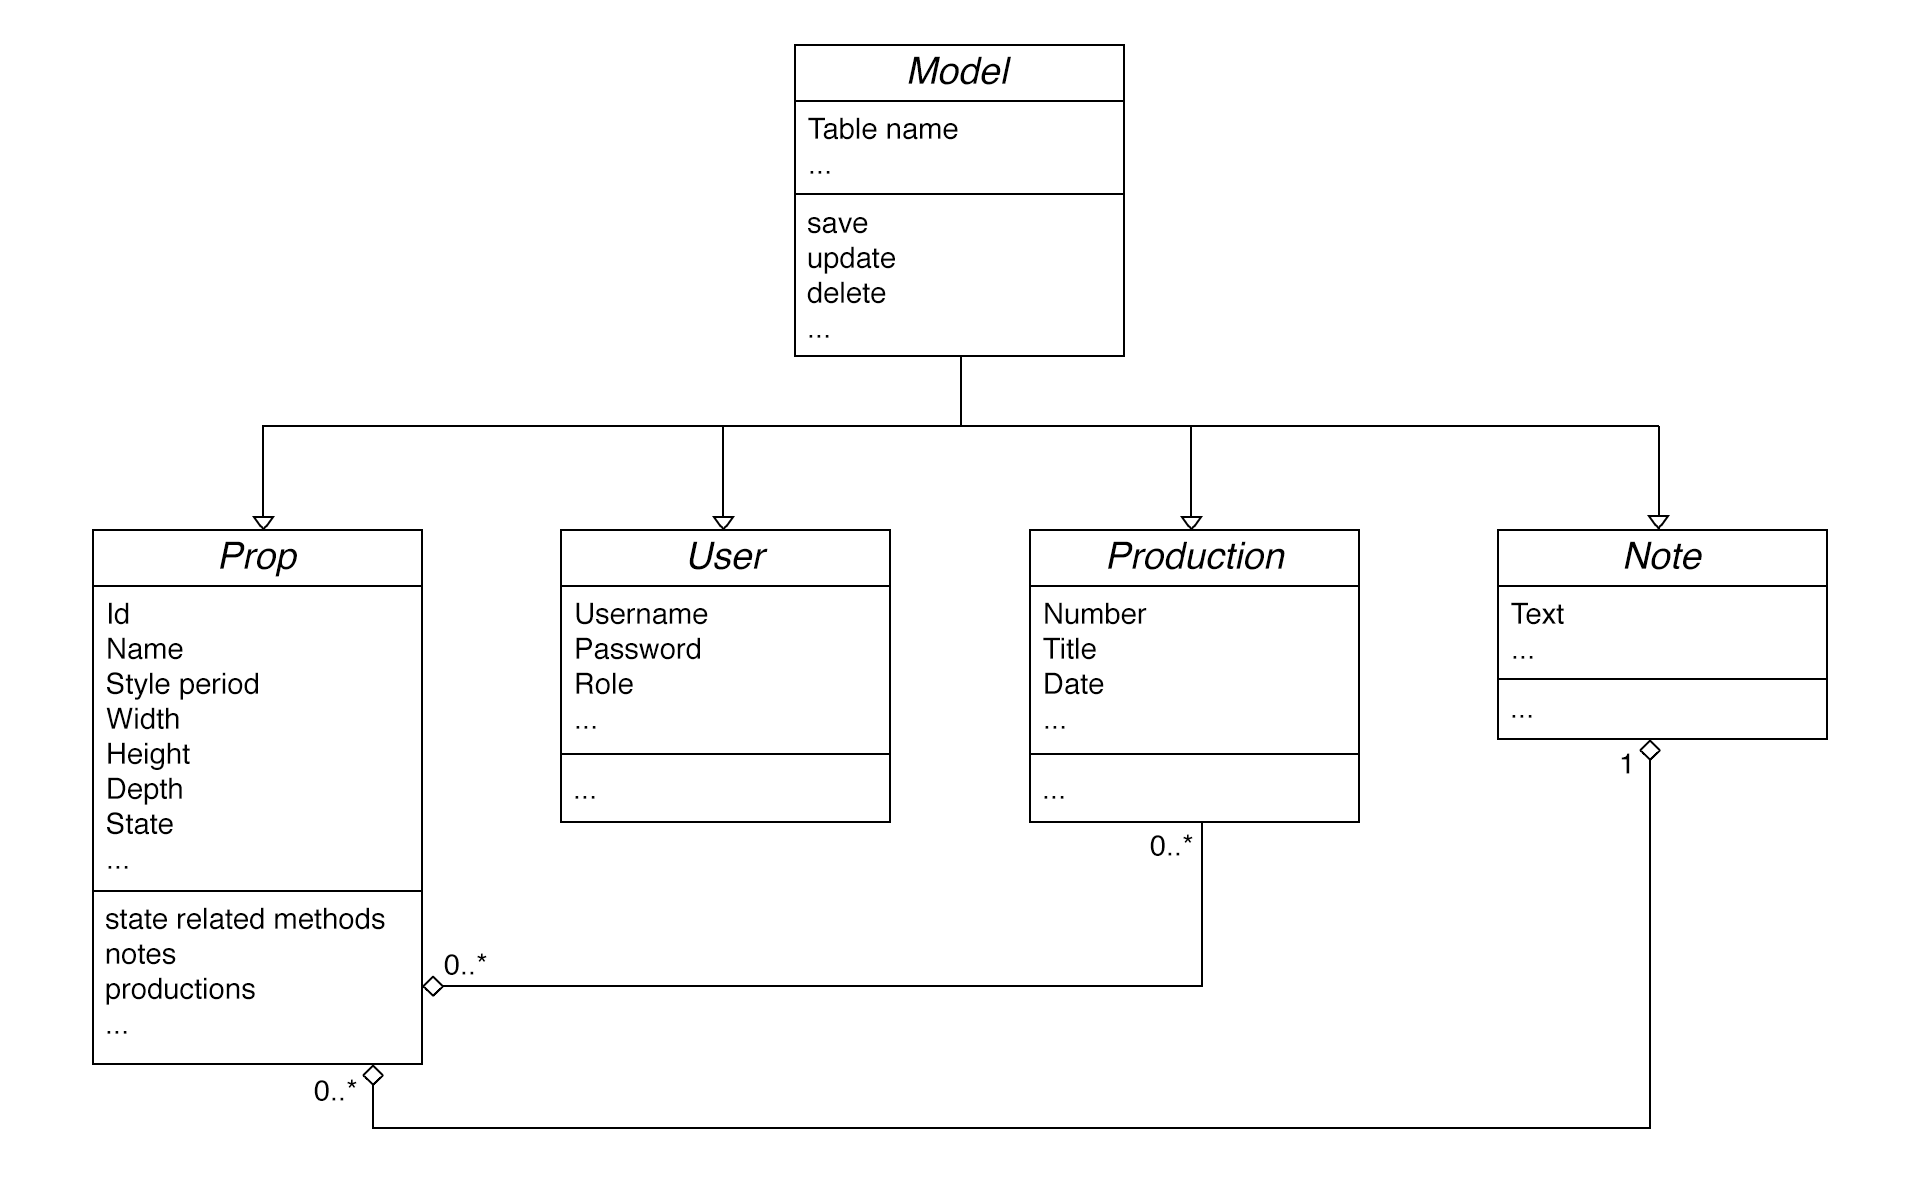
\includegraphics[scale=0.2]{class-diagram.png}
\newline
\newline
There will be one abstract model class that implements methods used by all models. There will then be subclasses of this model that implement the domain functionality.\\
They will be associated with each other in different ways. A prop will be associated with many productions and can have many notes. A production can have many props and a note belongs to exactly one prop.\\
There will then also be various attributes on the models that correspond to the database columns. The models will also have methods but at this point its hard to say specifically which methods they will need. The prop model will however most likely need methods for changing its state and accessing the other associated objects.
\section{System-design summary}
As we have not started coding yet a summary of the system-design so far, will be very abstract. So far we have used a lot of resources on the initial planning, both internal in the group, and in cooperation with the client, to ensure that our initial design-plan meets the expectations the client have for the new system. This has been a some what difficult task, as the new system will cause the client to change how they administratively handle the props. \\ 
Right now our main tasks will be to create the mySQL database, which involve transferring all of the data in the current system to our new system and adapt it to the fit the new database-design. We will, when possible, in this process, begin the PHP-coding and in that way develop back- and front-end simultaneously.  
\section{Program- and system-test}
The amount of testing we have done at this moment is very limited because we don't have any code yet to test. We have however discussed how we will structure the testing when we start coding.
\newline
\newline
We intend to use Test Driven Development when developing the system. This means that tests will be written before the implementation code is written. This weaves the test plan and implementation plan together. There will not be a dedicated time period in which we do the testing and there will not be a defined set of resources (developers) in charge of doing the testing. People will test their code as they write it and modify the tests accordingly when changing the code.
\newline
\newline
We don't have any test case specifications, a test incident report, or a test report summary, since we don't yet have any tests.
\section{User interface and interaction design}
\subsection{a) Screenshots of user interfaces}
% (a) Præsenter skærmbilleder af de mest interessante dele af jeres brugergrænseflade.
The following are screenshots of our most recent prototype.
\newline
\newline
\centerline{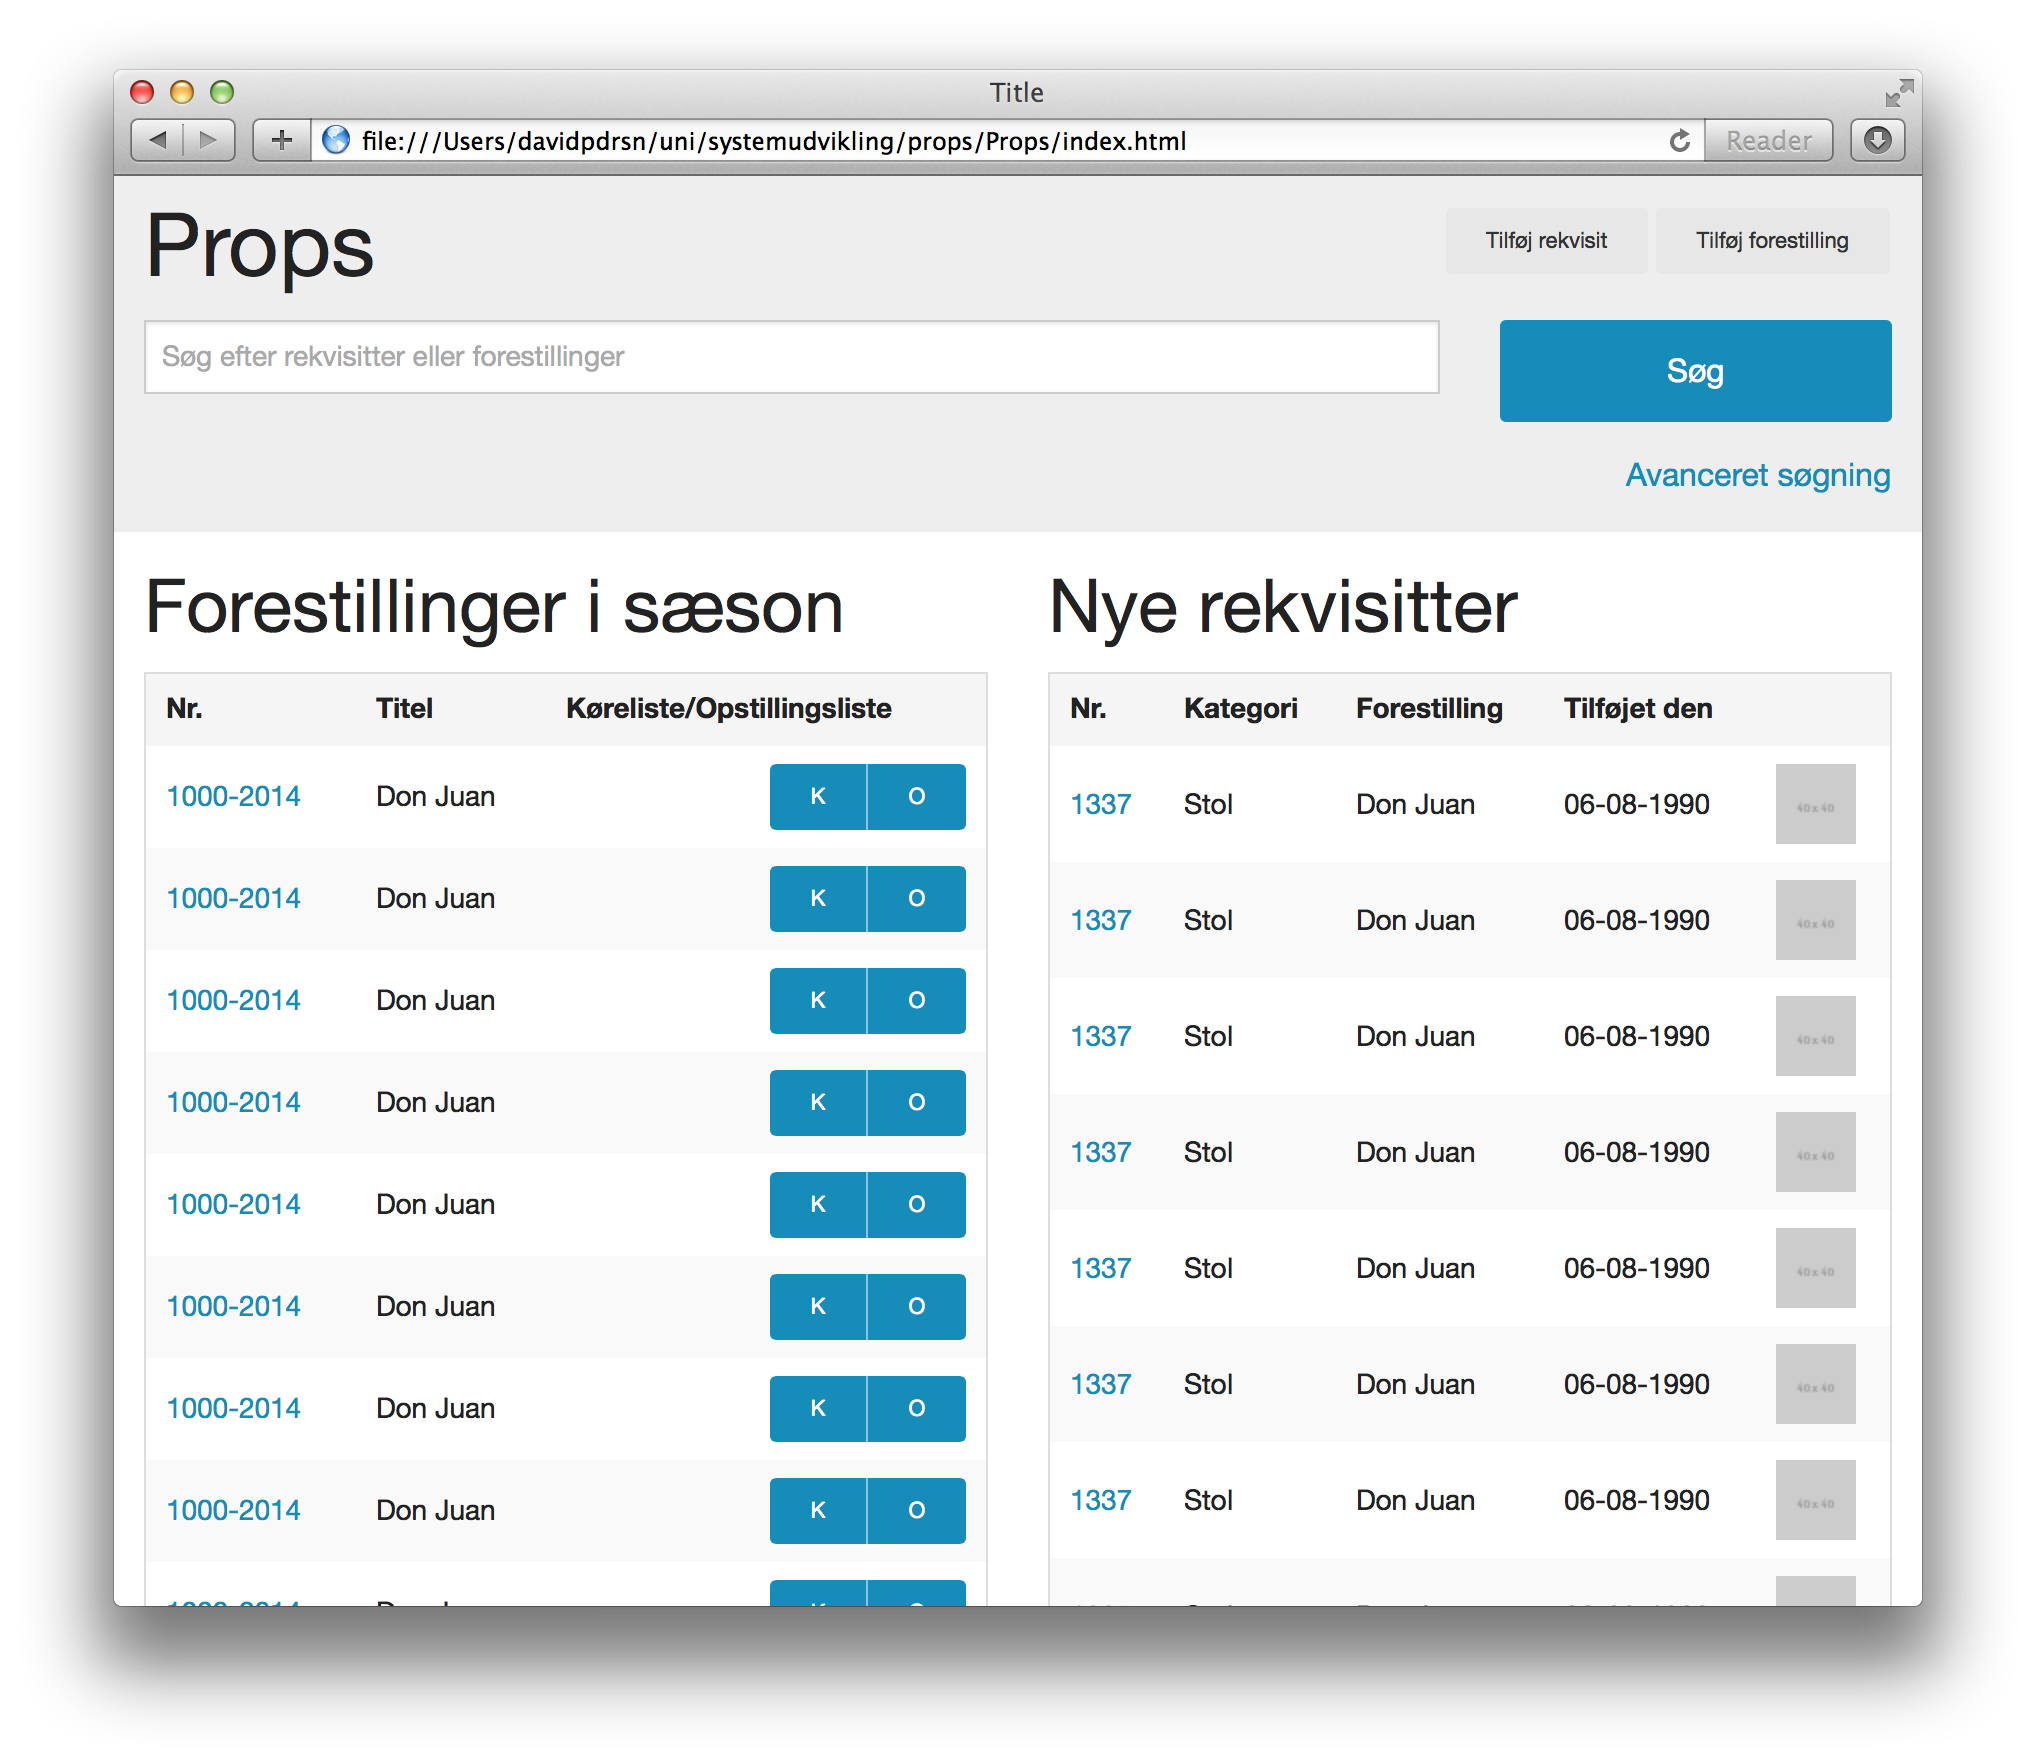
\includegraphics[scale=0.25]{prototype_frontpage.png}}
\newline
\textbf{Front page}\\
All pages will show a big search field up top as this is the primary feature of the site.\\
The frontpage also shows a list of productions that are being done this season as well as the latest props added to the database.
\newline
\newline
\centerline{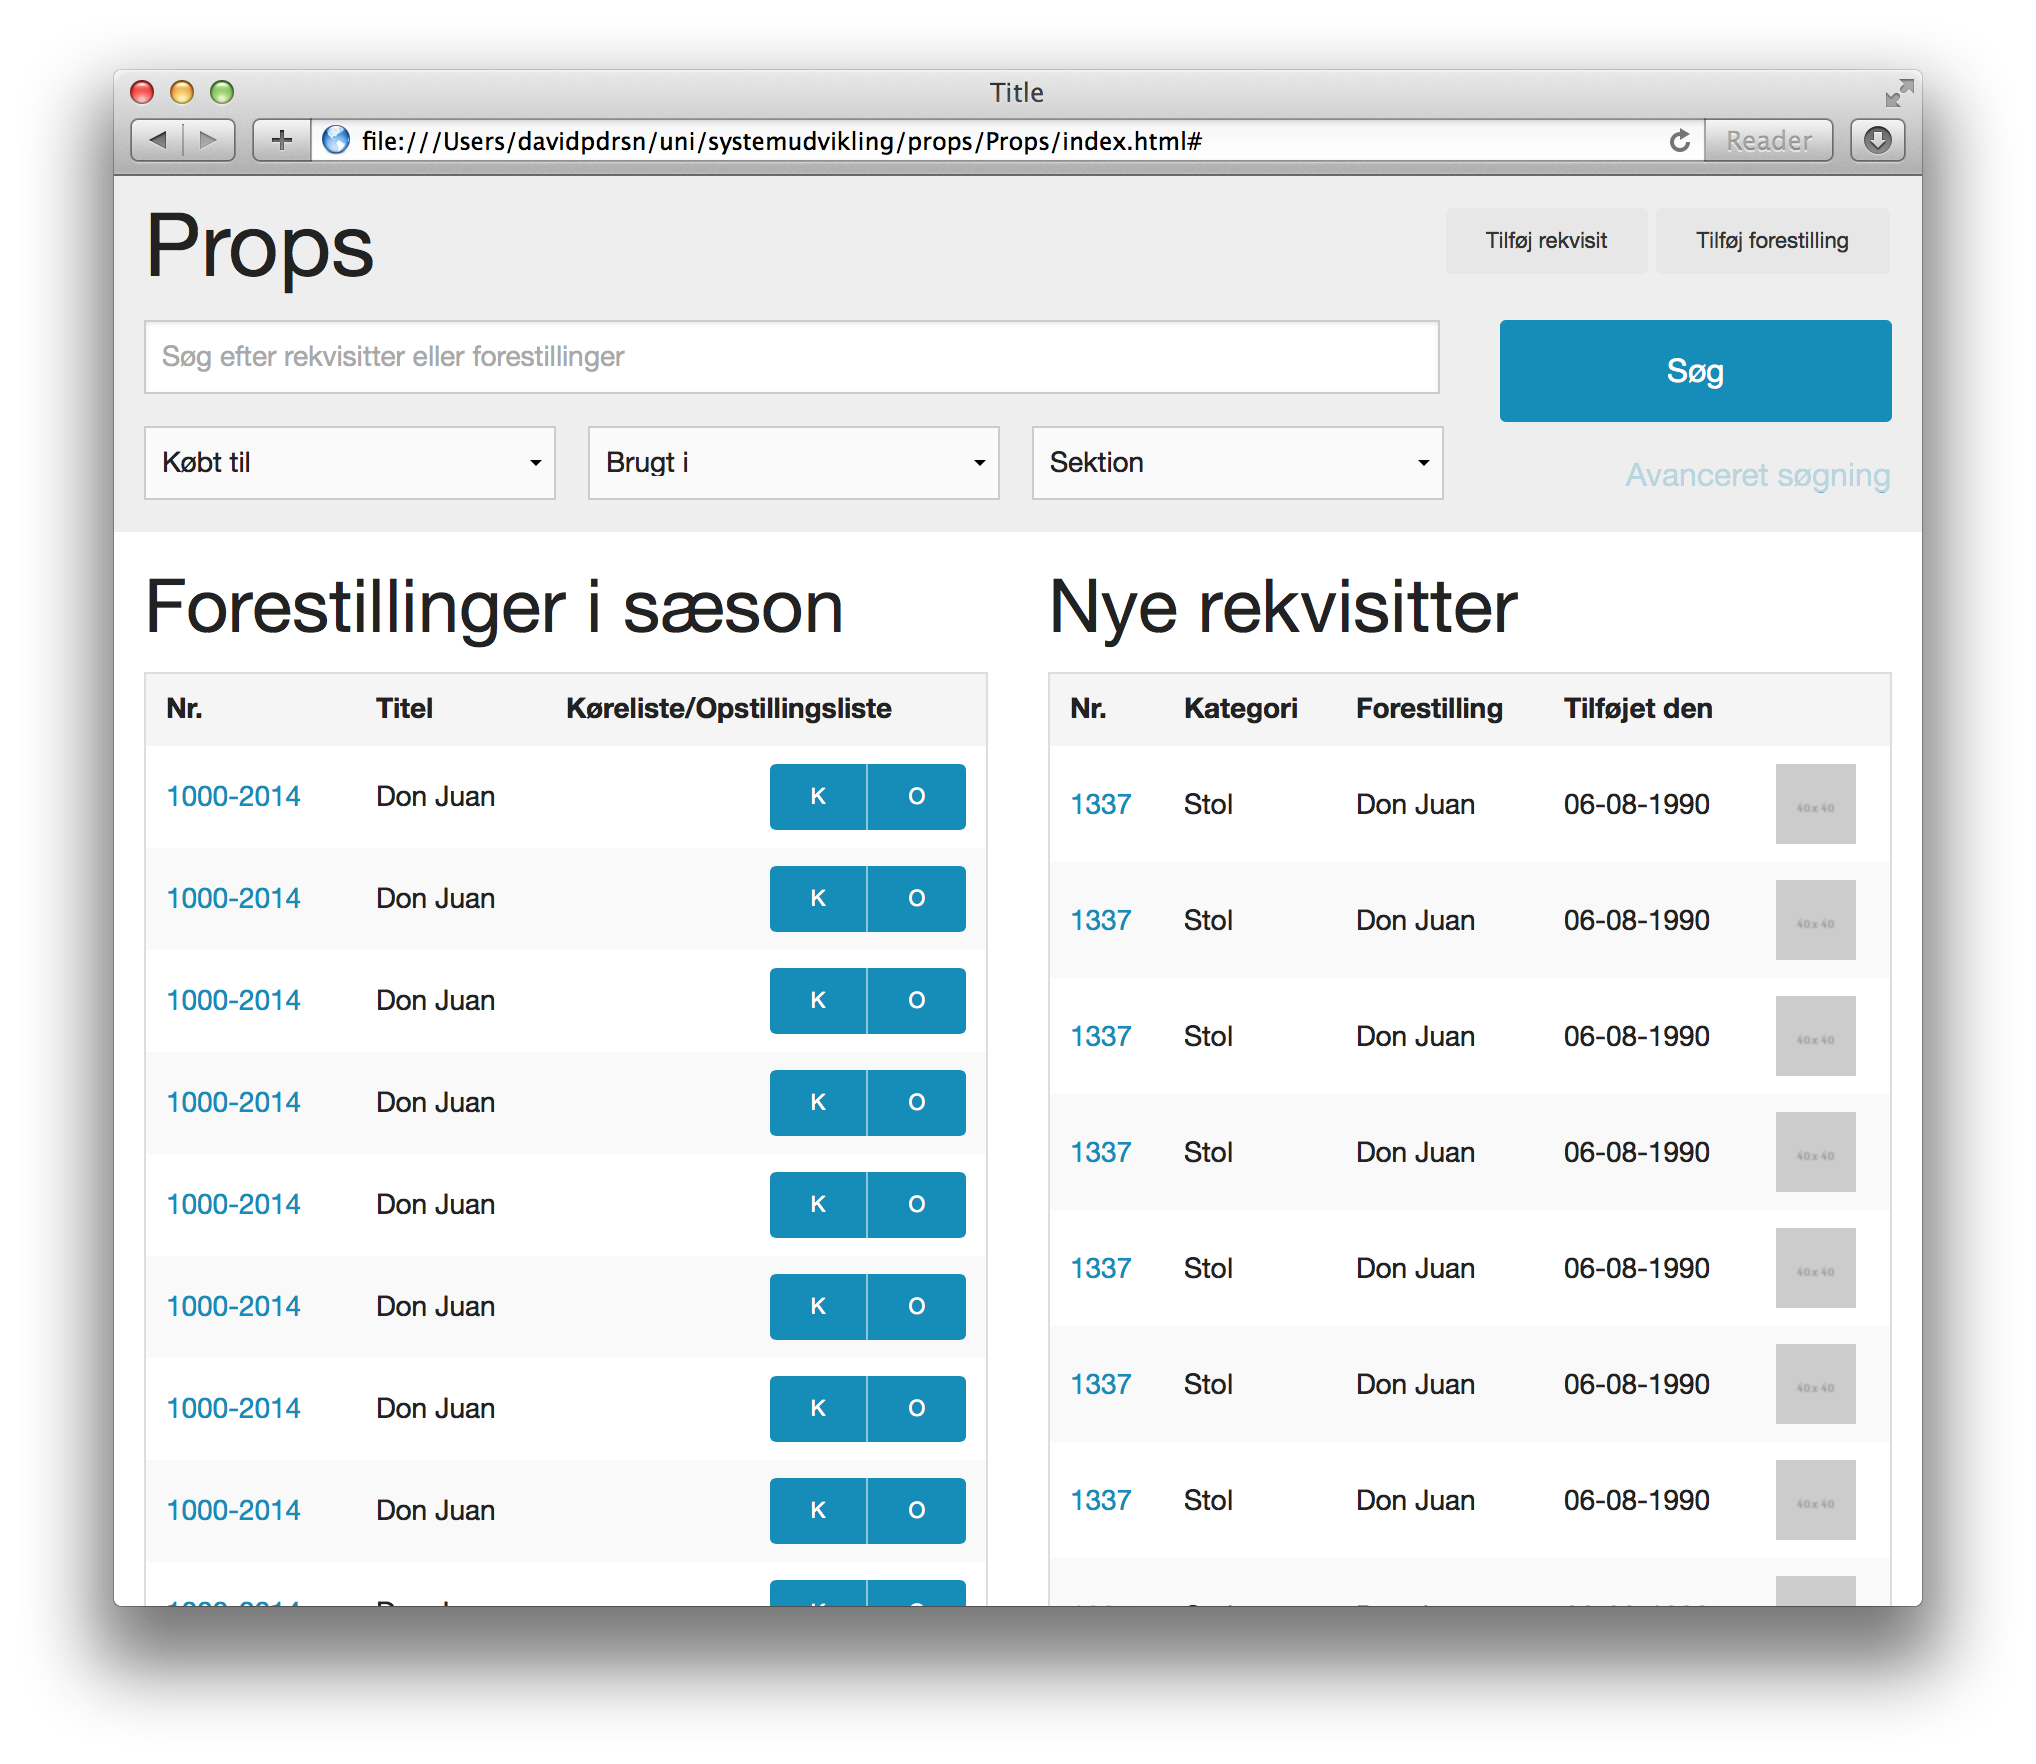
\includegraphics[scale=0.25]{prototype_advanced_search.png}}
\newline
\textbf{Front page with advanced search}\\
It is often useful to limit the scope of a search to a specfic production or a specific section of props. This can be done through some dropdown menus that appear when clicking on advanced search.
\newline
\newline
\centerline{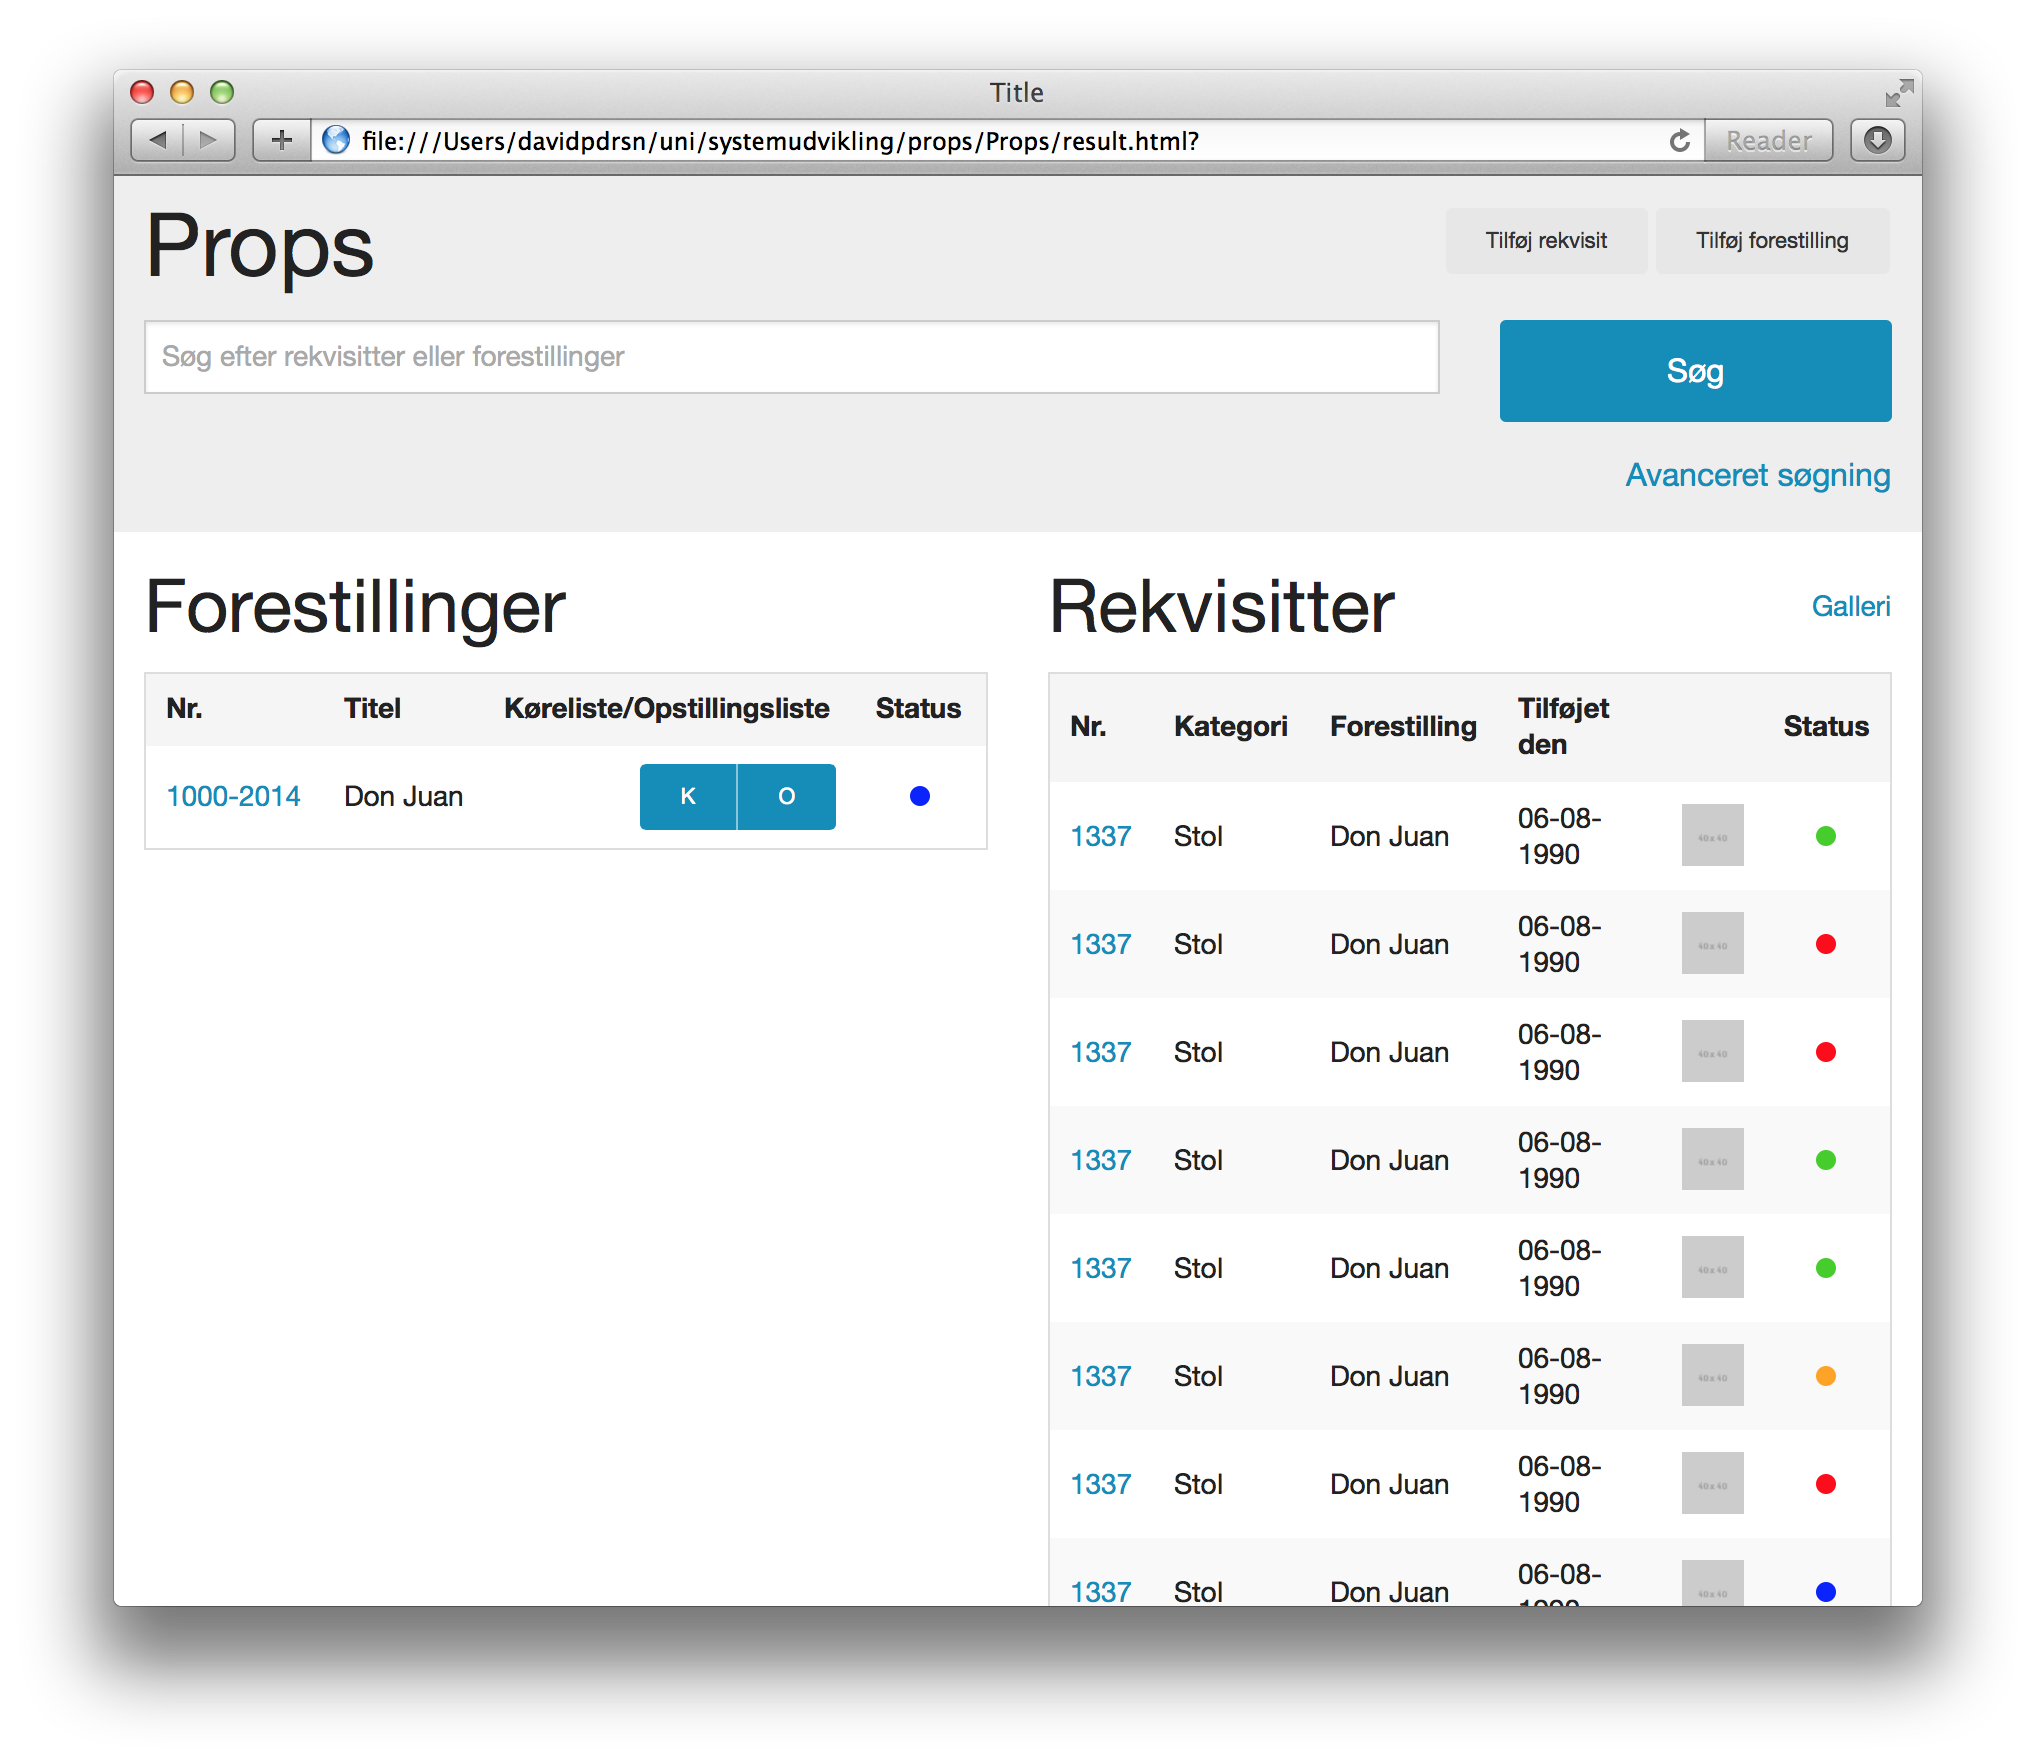
\includegraphics[scale=0.25]{prototype_search_result.png}}
\newline
\textbf{Search result page}\\
This page shows the result of doing a search. It shows the performances and props that were matched. Along with the attributes also shown on the frontpage it also shows the status of the prop and production. A status could be something like "reversed" or "free to use".
\newline
\newline
\centerline{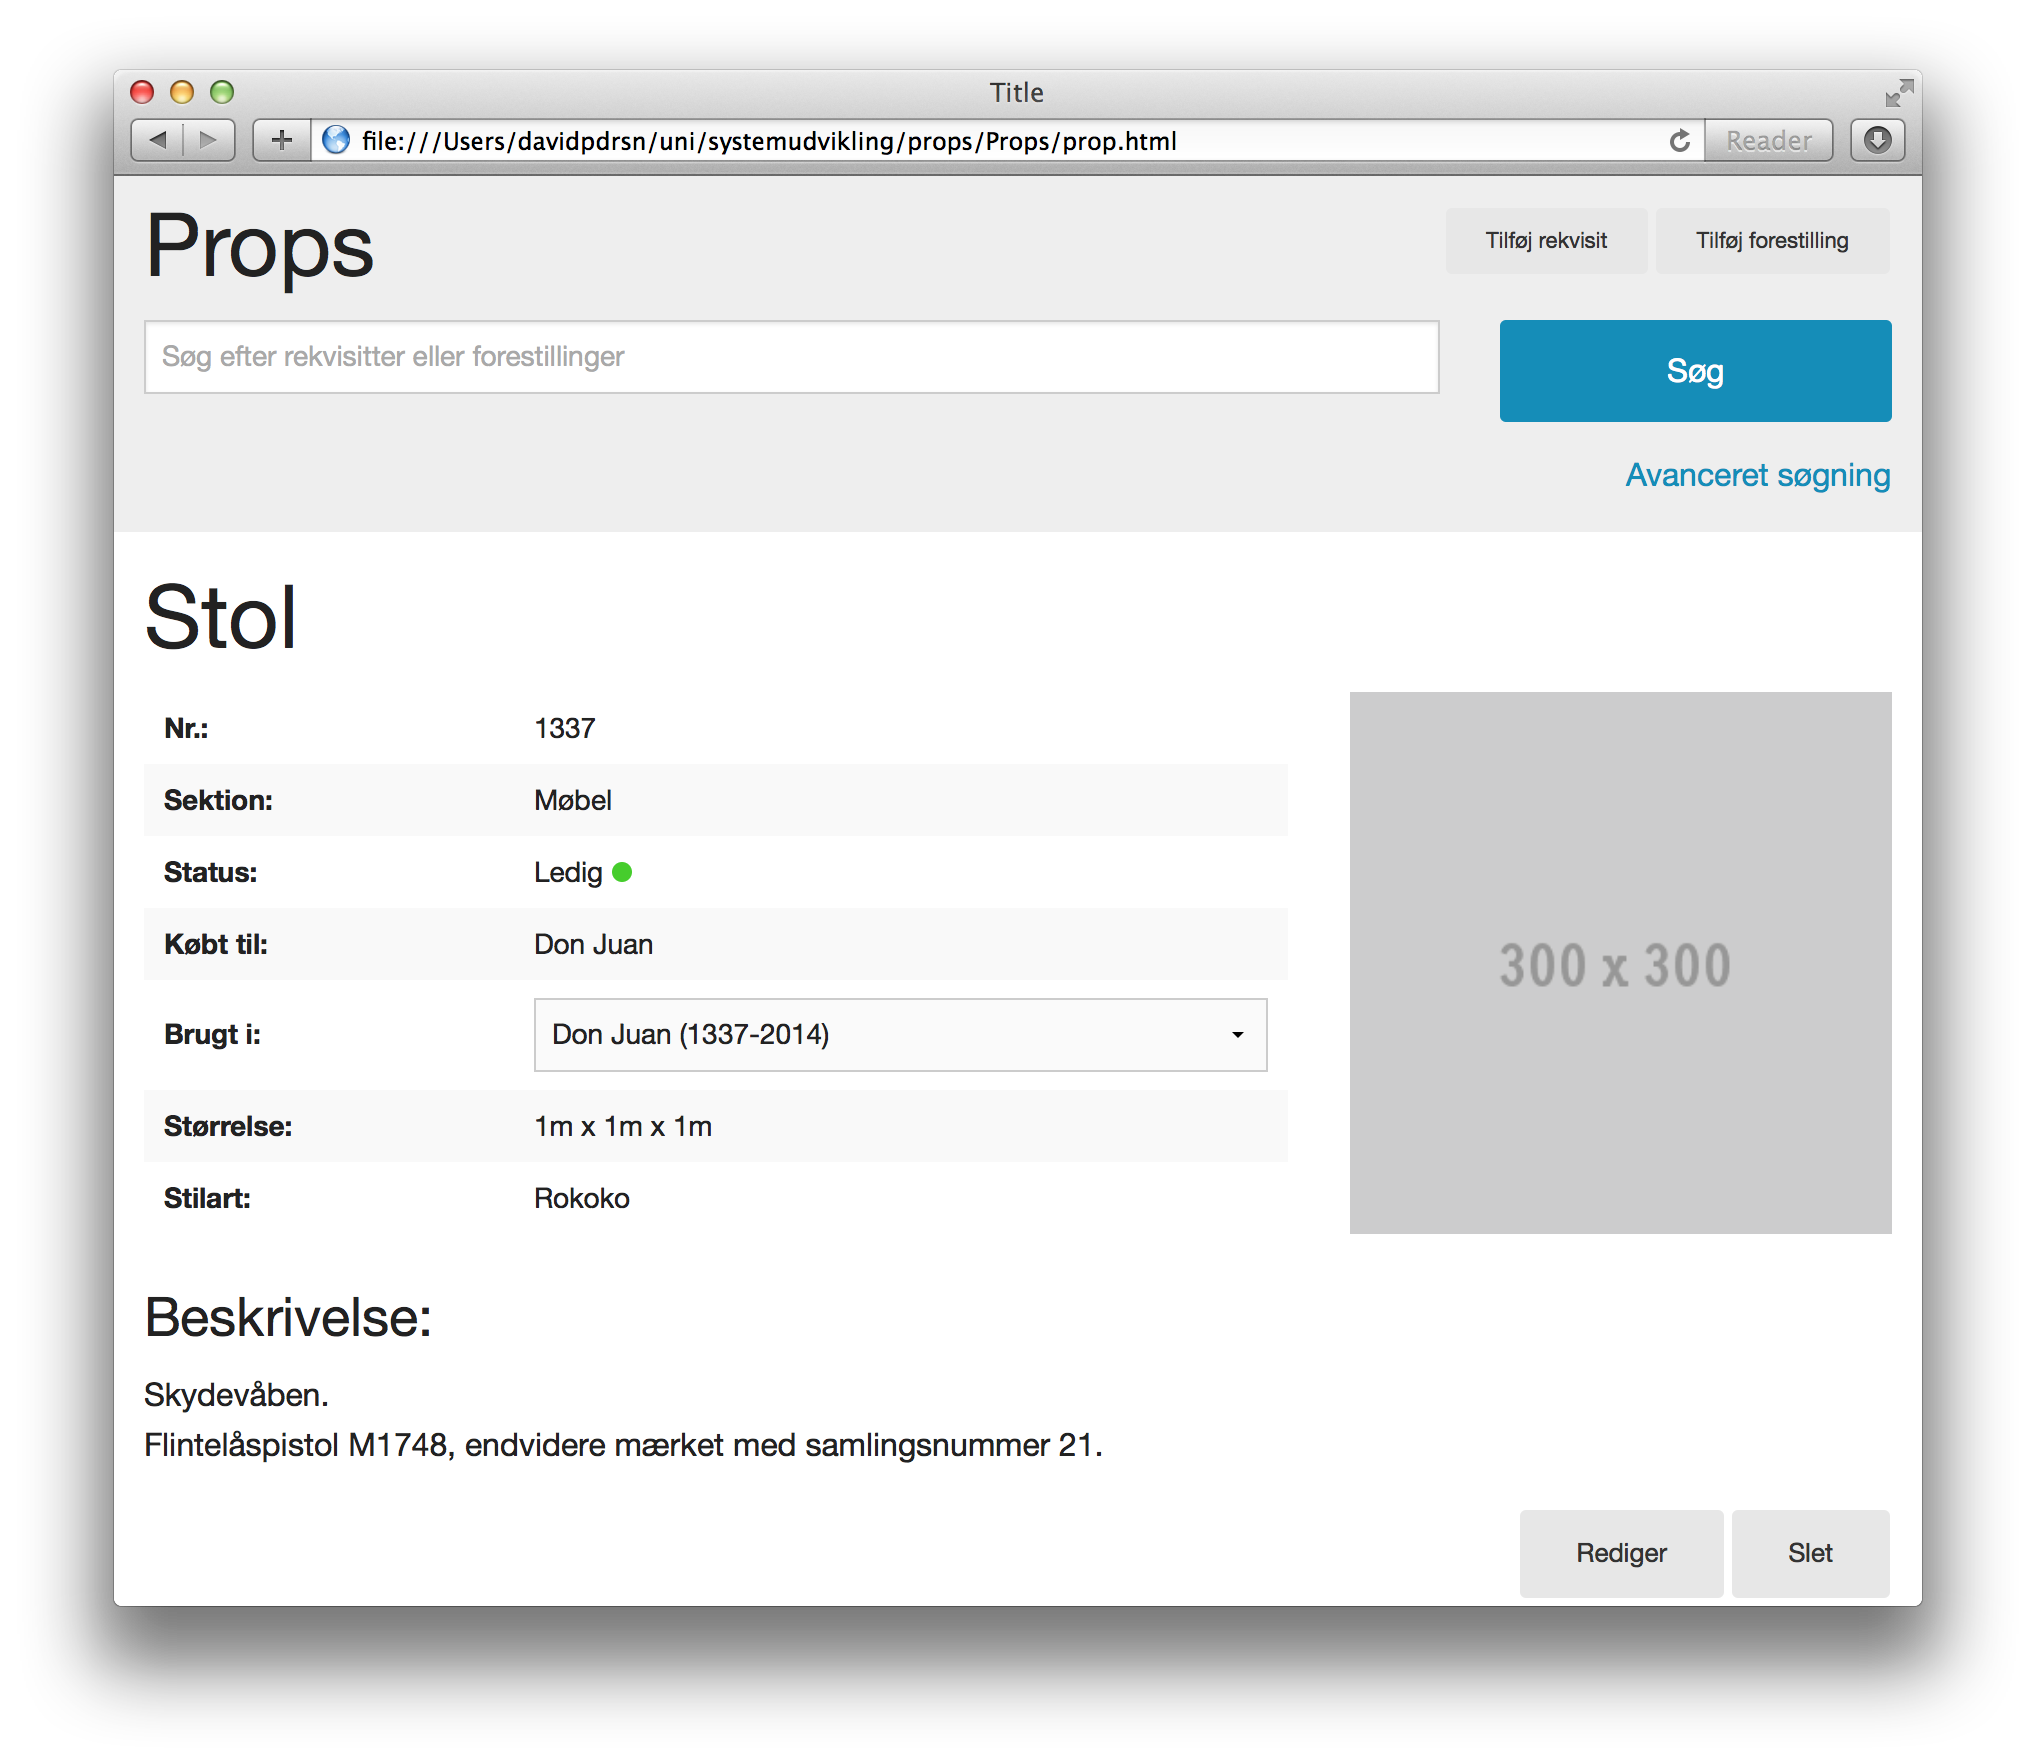
\includegraphics[scale=0.25]{prototype_show_prop.png}}
\newline
\textbf{Single prop page}\\
This is the page the shows information about a single prop in the database. It simply shows the attributes of the prop.
\subsection{b) Flow and user interactions}
The prototype we have is just static HTML files so there are no dynamics to illustrate, yet.
\subsection{c) Demo of prototype}
There is no actual behavior to give a demonstration of yet.
\subsection{d) Review of latest think aloud test}
We have not conducted any user tests.
\section{Version control}
We have not yet started implementing any part of the system so we have no version control history to discuss.
\section{Project collaboration}
% Til aflevering: Beskriv konkret og oplysende hvordan det går med samarbejdet med brugerne og med arbejdet internt i gruppen. Herunder skal bl.a. oplyses antallet af møder med brugerne under projektforløbet (fx på en tidslinje), mødeformen i gruppen, samt hvorledes jeres referat- og dokumentationsform fungerer. Hvorledes prioriterer og styrer I projektindsatsen, så I sikrer fremdrift på de felter, som er mest risikable/afgørende for et succesfuldt resultat? Herunder, beskriv og diskuter:
\subsection{a) What's going well?}
% (a) Hvad går godt?
...
\subsection{b) What's going less well?}
% (b) Hvad går mindre godt?
...
\subsection{c) Improving the collaboration}
% (c) Hvad vil I gøre for at effektivisere jeres udviklingsarbejde?
...
\end{document}
